\SECTION{Design and Implementation}\label{sec:design_imple}
In this section, we present the design and implementation of Linux-RTXG,
which achieves a real-time GPU scheduling framework without kernel modification.
We describe the main contribution of the GPU scheduler and its integration to a CPU scheduler.
Note that the discussion of CPU scheduling is minimized because Linux-RTXG is based on RESCH.

\SUBSECTION{Linux-RTXG}
\begin{figure}[t]
\begin{center}
\ifthesis
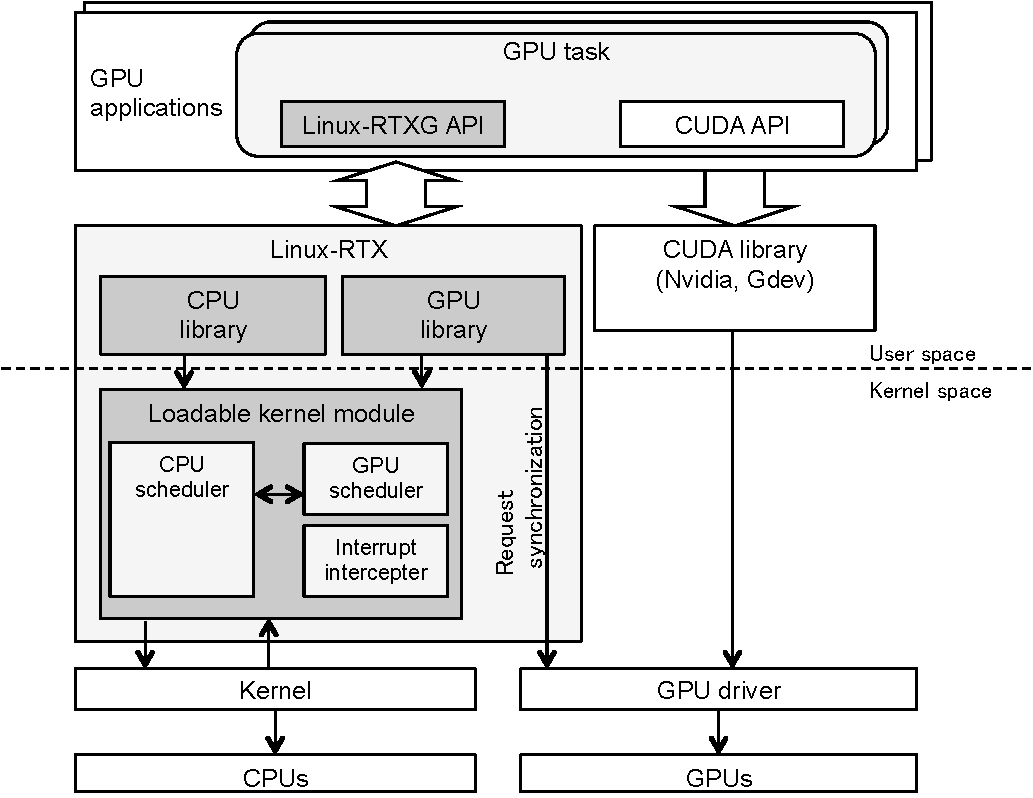
\includegraphics[width=0.8\textwidth]{img/overview.pdf}
\else
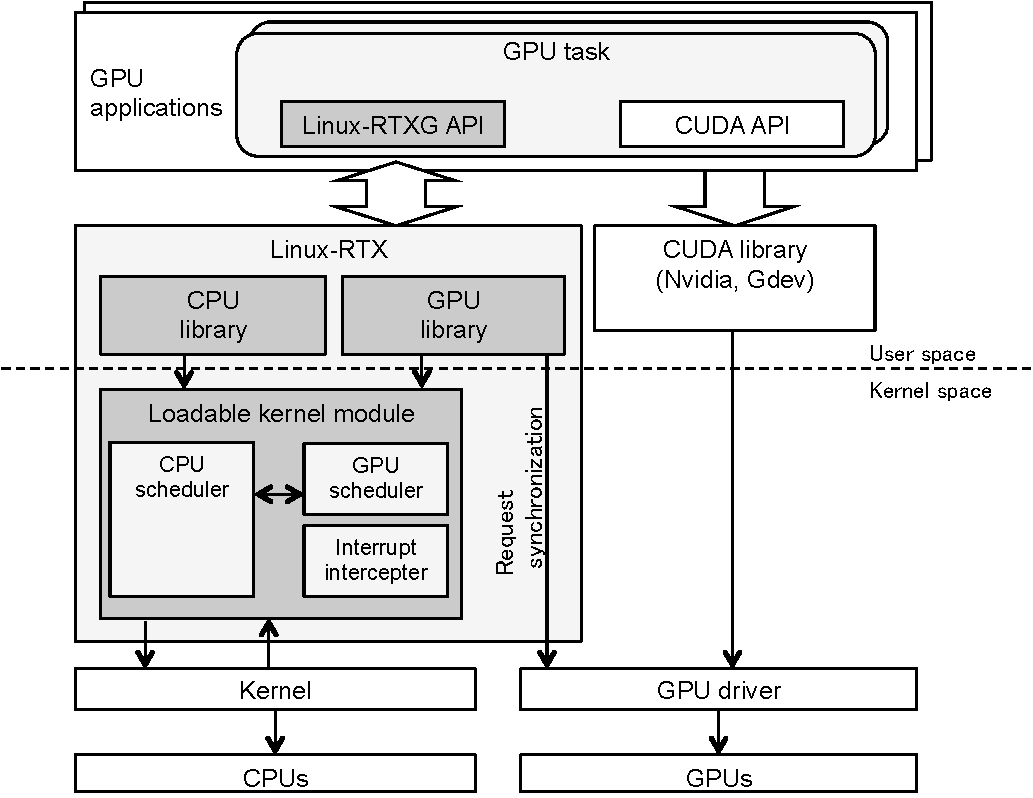
\includegraphics[width=0.35\textwidth]{img/overview.pdf}
\fi
\caption{Overview of Linux-RTXG}
\label{fig:overview}
\end{center}
\end{figure}

Figure~\ref{fig:overview} shows an overview of Linux-RTXG.
Linux-RTXG is divided into two parts, the core and the library.
The Linux-RTXG core has a CPU task scheduler, a GPU task scheduler, and a GPU resource reservation mechanism.
The Linux-RTXG core is loaded into kernel-space; thus, it can use exported kernel functions, such as $schedule()$, $mod\_timer()$, $wake\_up\_process()$, and $set\_cpus\_allowed\_ptr()$.
These interfaces are implemented using an input/output control(ioctl) system call, which is a standard way of communicating with a driver.
The library includes an independent synchronization method.
The independent synchronization method is used only on the NVIDIA driver.
If using an open-source GPU driver, such as Nouveau~\cite{nouveau}, GPU runtime must use part of Gdev.
Gdev can manage arbitrary interrupts of the GPU kernel in the user-space mode;
therefore, the GPU scheduler does not require independent synchronization.
\SUBSECTION{GPU Scheduling}
\begin{table*}[!t]
\begin{center}
\caption{Basic Linux-RTXG APIs}
\label{tab:rtx-api}
\ifthesis
\begin{tabular}{|l|p{25em}|} \hline
\else
\begin{tabular}{|l|p{50em}|} \hline
\fi
rtx\_gpu\_open() & Registers itself to Linux-RTXG and creates scheduling entity. It must be called first. \\ \hline
rtx\_gpu\_device\_advice() & Obtains recommendations for which GPU devices to use. \\ \hline
rtx\_gpu\_launch() & Controls GPU kernel launch timing, (i.e., a scheduling entry point). It must be called before the CUDA launch API. \\ \hline
rtx\_gpu\_sync() & Waits for the completion of GPU kernel execution by sleeping with TASK UNINTERRUPTIBLE status. \\ \hline
rtx\_gpu\_notify() & Sends NOTIFY/FENCE command to GPU. The FENCE/NOTIFY are selected by flag that is set by argument.\\ \hline
rtx\_gpu\_close() & Releases scheduling entity.\\ \hline
\end{tabular}
\end{center}
\end{table*}

Linux-RTXG is a scheduler that a combination of an API-driven and interrupt-driven.
The scheduler is invoked only when computation requests are submitted.
The basic APIs supported by Linux-RTXG are listed in Table~\ref{tab:rtx-api}.
Note that some APIs have arguments and others do not.
Linux-RTXG does not modify the existing CUDA API to cope with proprietary software in order to be independent of GPU runtime.
However, the user must add the Linux-RTXG API to existing CUDA applications to use the Linux-RTXG scheduler.

Sample Linux-RTXG scheduler code is shown in Figure~\ref{fig:sample}.
GPU tasks are provided with a function by calling Linux-RTXG's API at strategic points.

\begin{figure}[!t]
\begin{center}
\begin{tabular}{l}
\hline\hline
{\scriptsize \verb|void gpu_task(){        |}\\
{\scriptsize \verb| /* variable initialization  */        |}\\
{\scriptsize \verb| /* calling RESCH API */        |}\\
{\scriptsize \verb|  dev_id = rtx_gpu_device_advice(dev_id); |}\\
{\scriptsize \verb|  cuDeviceGet(&dev, dev\_id);           |}\\
{\scriptsize \verb|  cuCtxCreate(&ctx, SYNC_FLAG, dev);    |}\\
{\scriptsize \verb|  rtx_gpu_open(&handle, vdev_id);     |}\\
{\scriptsize \verb| /* Module load and set kernel function */ |}\\
{\scriptsize \verb| /* Device memory allocation        */ |}\\
{\scriptsize \verb| /* Memory copy to device from host */ |}\\
{\scriptsize \verb|  rtx_gpu_launch(&handle); |}\\
{\scriptsize \verb|  cuLaunchGrid(function, grid_x, grid_y); |}\\
{\scriptsize \verb|  rtx_gpu_notify(&handle); |}\\
{\scriptsize \verb|  rtx_gpu_sync(&handle);   |}\\
{\scriptsize \verb|  /* Memory copy to host from device */  |}\\
{\scriptsize \verb|  /* Release allocated memory */  |}\\
{\scriptsize \verb|}|}\\
\hline\hline
\end{tabular}
\caption{sample code of using Linux-RTXG scheduler}
\label{fig:sample}
\end{center}
\end{figure}

\begin{figure}[!t]
\begin{center}
\ifthesis
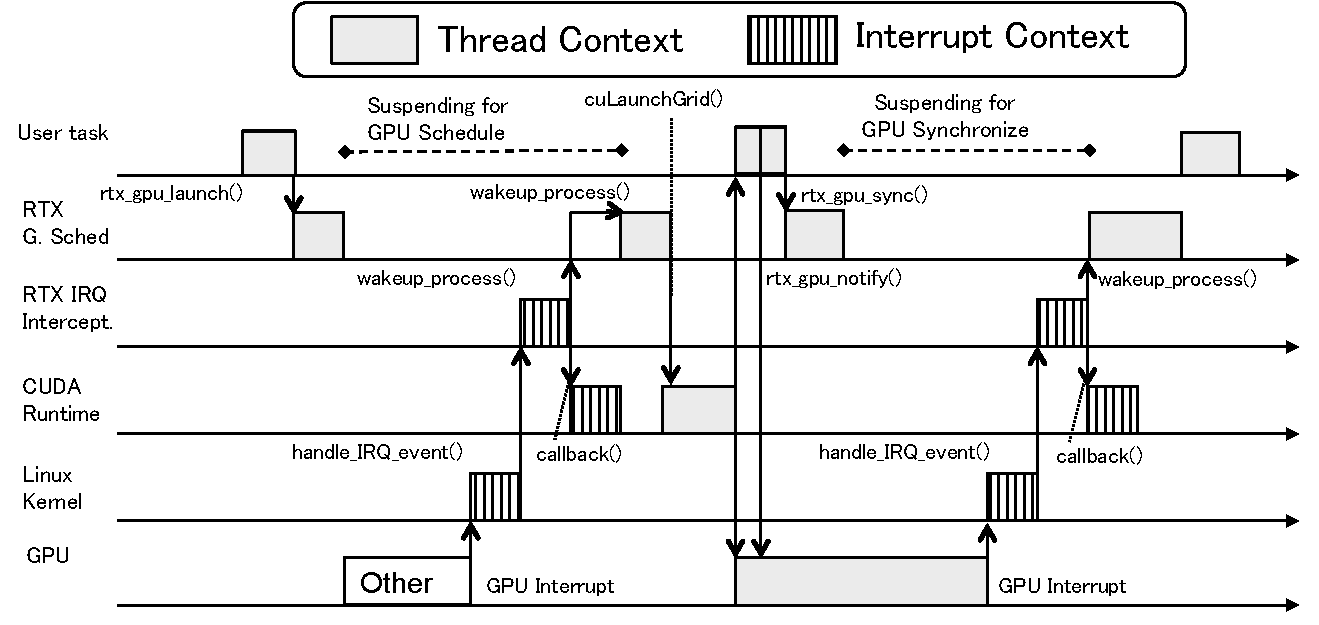
\includegraphics[width=\textwidth]{img/gsched_controlflow.pdf}
\else
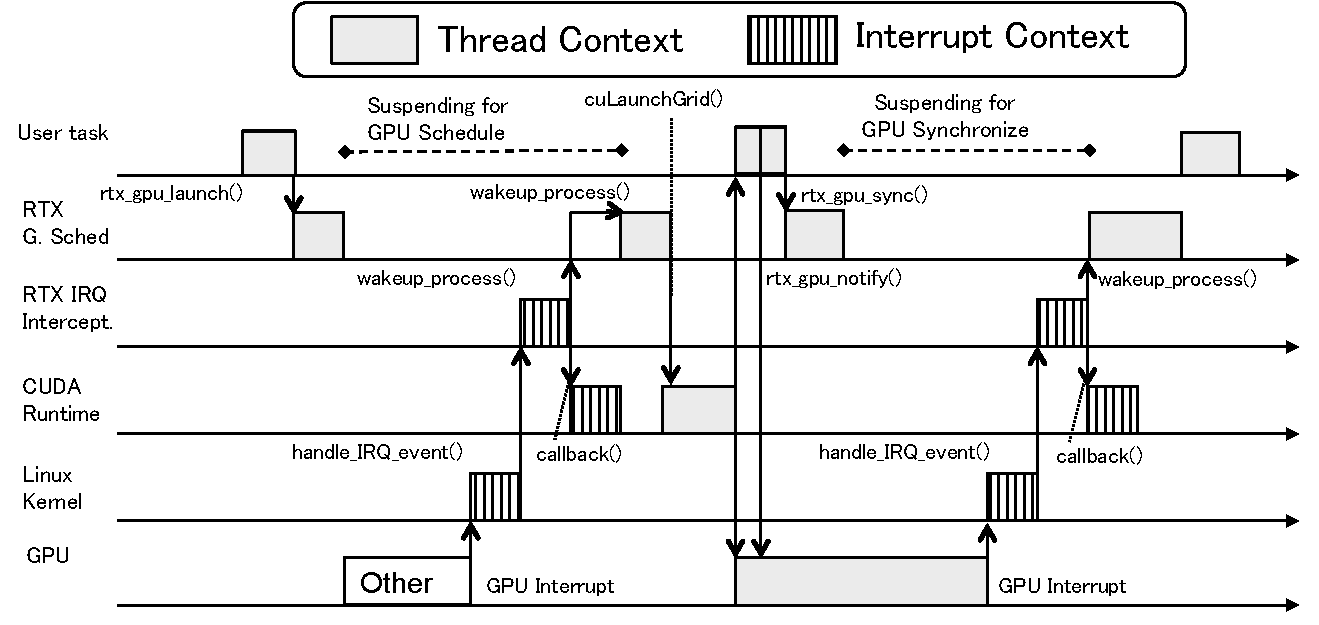
\includegraphics[width=0.5\textwidth]{img/gsched_controlflow.pdf}
\fi
\caption{GPU Scheduling control flow}
\label{fig:controlflow}
\end{center}
\end{figure}

In Figure~\ref{fig:controlflow} is restricted to a single GPU kernel.
A GPU task can control the timing of the GPU kernel execution by calling $rtx\_gpu\_launch()$.
The task sleeps until it receives an interrupt because an additional GPU kernel cannot be issued until a current task completes execution.
When the current task's GPU kernel completes execution, the Linux kernel handles the interrupt.
The interrupt interceptor then wakes the sleeping task.
The woken task is issued the GPU kernel via a CUDA API, such as $cuLaunchGrid()$.
After the GPU kernel is issued, the task registers NOTIFY to monitor interrupt,
and is put to sleep until it receives an interrupt.
Selection of the subsequent task is performed by the GPU scheduler caused by the interruption of GPU kernel finish.
Linux-RTXG controls the order of task execution according to the above flow.

We present a hierarchal scheduling that includes group (virtual GPU) scheduling and GPU kernel scheduling.
The virtual GPU scheduling uses a resource reservation mechanism.
The GPU kernel scheduling uses a fixed-priority scheduling.
Specifically, GPU kernel execution is associated with each scheduling entity while Linux-RTXG groups scheduling entity to virtual GPUs.
The virtual GPUs can belong to any of the physical GPUs.
In Linux-RTXG, resources are distributed to virtual GPUs.

Figure~\ref{fig:scheduling} shows pseudo-code of the scheduling mechanism.
Here, $on\_arrival$ is called when a GPU task is requested GPU kernel launch.
In $on\_arrival$, a GPU task checks whether the given executions permission to virtual GPU of task itself, and then check the $se$ permit.
If a virtual GPU to which the GPU task belongs has not executing permission, the GPU task is queued to wait\_queue and is suspended (i.e., it is put to sleep).
If the virtual GPU has execution permission, the GPU task is launched.
$on\_completion$ is called by a scheduler thread when the execution of the GPU kernel is complete.
$on\_completion$ selects up the next virtual GPU and the next GPU task.
Next, $on\_completion$ wakes the selected GPU task.

\begin{figure}[!t]
\begin{center}
\begin{tabular}{l}
\hline
{\scriptsize \verb| se: The scheduling entity |}\\
{\scriptsize \verb| se->vgpu: The group that is belonged se|}\\
{\scriptsize \verb| se->task: The task that is associated with se |}\\
{\scriptsize \verb| vgpu->parent: The physical GPU identification|}\\
\hline
{\scriptsize \verb|void on_arrival(se) {|}\\
{\scriptsize \verb| check_permit_vgpu(se->vgpu)    |}\\
{\scriptsize \verb| while(!check_permit_se(se)){|}\\
{\scriptsize \verb|   enqueue(se->vgpu,se); |}\\
{\scriptsize \verb|   sleep_task(se->task); |}\\
{\scriptsize \verb|}}|}\\
{\scriptsize \verb|void on_completion(se) {|}\\
{\scriptsize \verb| reset_the_permit(se->vgpu, se)|}\\
{\scriptsize \verb| n_vgpu = pick_up_the_next_vgpu(se->vgpu->parent) |}\\
{\scriptsize \verb| se = pick_up_the_next_se(n_vgpu)|}\\
{\scriptsize \verb| if(se) {|}\\
{\scriptsize \verb|   dequeue(se->vgpu,se);|}\\
{\scriptsize \verb|   wakeup_task(se->task);|}\\
{\scriptsize \verb| }|}\\
{\scriptsize \verb| set_the_permit(se->vgpu, se)|}\\
{\scriptsize \verb|}|}\\
\hline
\end{tabular}
\caption{Scheduling mechanisms of high-level pseudo-code}
\label{fig:scheduling}
\end{center}
\end{figure}

\SUBSECTION{GPU Synchronization}
Here, we describe the independent synchronization mechanism and the interrupt intercept.
The independent synchronization mechanism invokes NOTIFY and FENCE without using a GPU runtime API.
The interrupt intercept realizes interrupt-driven wakeup of the scheduler without kernel modification.
Linux-RTXG uses the independent synchronization mechanisms as much as possible
because we do not want to use black--box resource management.

\textbf{Independent synchronization mechanism from runtime:}
We present an independent synchronization mechanism for NOTIFY and FENCE.
The mechanism invokes an interrupt for NOTIFY, and writes the fence value with the GPU microcontrollers for FENCE.
NVIDIA's proprietary software uses the ioctl interface to communicate between the kernel-space and the user-space.
These ioctl interfaces provide driver functions, such as device memory allocation, obtaining GPU information and memory mapping.
Gdev builds infrastructure that can execute on NVIDIA's driver using these ioctl interfaces.
The proposed method uses an ioctl interface similar to Gdev's method for sending commands.
Specifically, the proposed method is divided into two parts, Initialize and Notify.
Initialize processess generate a dedicated GPU context.
This processess include creating virtual address space, allocating an indirect buffer object for sending a command, and creating a context object is required to prepare the FIFO engine and includes, allocating a kernel memory object and mapping the FIFO engine register to host memory space using memory-mapped I/O.
The FIFO engine is a GPU microcontroller that receives commands.
The Notify processes send commands to a compute engine or a copy engine by $iowrite$ function to the mapped FIFO engine's register.
The compute engine and the copy engine do function that switching a GPU context for computing or data copy.
This independent synchronization mechanism uses reverse engineering.
Therefore, this method depends on the GPU device architecture and the proprietary software interfaces.

\textbf{Interrupt interception:}
Interrupts are handled by the ISR registered to the kernel by the device driver.
In addition, a scheduler is required to receive the interrupt and to identify the interrupt by reading the GPU status register.
The GPU status register must be read before the original ISR resets the GPU status register.

The Linux kernel has structures that hold interrupt parameters called $irq\_desc$ for each interrupt number.
These structures have structures called $irq\_action$, including the ISR callback pointer.
An $irq\_desc$ is allocated to global kernel memory space, and is freely accessible from kernel space.
Linux loadable kernel modules can obtain an $irq\_desc$ and an ISR callback pointer.
We obtain the GPU device driver's ISR callback pointer, and then we register an interrupt interception ISR to the kernel.
Thus, we obtain an interrupt interception from the interrupt interception ISR and retain the callback pointer.
In addition, I/O registers are mapped to kernel memory space by the device driver from the PCIe base address registers (BAR)~\cite{fujii:icpads2013,kato2013zero}.
Therefore, Linux-RTXG remaps the BAR0 to our allocated space using $ioremap()$ when the ISR initialized.
The interrupt interception identifies an interrupt by reading this mapped-space.

\SUBSECTION{Scheduler Integration}
The native Linux scheduler has various real-time scheduling policies, such as $SCHED\_DEADLINE$, $SCHED\_FIFO$ and $SCHED\_RR$.
$SCHED\_DEADLINE$ is an implementation of a constant bandwidth server and a global earliest deadline first.
$SCHED\_DEADLINE$ is included in the Linux 3.14.0 kernel.
However, synchronization does not work well with the SCHED\_DEADLINE scheduling policy for GPU tasks.
Here there are two problems.
The first is the implementation of $sched\_yield$---.$sched\_yield()$ uses $yield()$ in kernel space---.
The second is the implementation of waking from a sleeping state.

The first problem occurs by releasing the CPU using $sched\_yield()$ while waiting for I/O in polling.
Polling (spin) is the exclusive CPU; therefore, a task may once better to release the CPU can obtain good results.
However, $sched\_yield$ will set the polling task's remaining execution time to 0 by treating it as a parameter of $SCHED\_DEADLINE$.
Thus, the task cannot execute until the runtime is replenished in the next period.
Therefore, the task cannot call $sched\_yield()$ between polling.
$sched yield()$ is frequently used by device drivers and libraries, as well as GPU environment, and such software is affected by this problem.
Depending on the setting, even NVIDIA's CUDA can be affected by this problem.
We address this problem by limiting the GPU synchronization method to NOTIFY in the $SCHED\_DEADLINE$ policies.

The second problem is subjected to a check equation~\ref{eq} when restoring a task from the sleep state.
If equation~\ref{eq} holds, the runtime is replenished and absolute deadline is set to the next cycle deadline.

{\scriptsize
\begin{equation}
\frac{Absolute\_Deadline - Current\_Time}{Remaining\_Runtime} > \frac{Relative\_Deadline}{Period} \label{eq}
\end{equation}
}

We implement this check by subtracting GPU execution time from $Remaining Runtime$ when a task is restored by GPU kernel execution, with the exception of a task that is restored by period.
